%document.tex
\documentclass[UTF8, onecolumn, a4paper]{article}
\def\allfiles{}
\usepackage{ctex}
\setlength{\parindent}{2em}
\usepackage{appendix}
\usepackage{geometry}
\usepackage{amsmath, amsthm}
\usepackage{multirow, multicol}
\usepackage{subfigure}
\usepackage{float}
\usepackage{graphicx}
\usepackage{lettrine}
\usepackage{authblk}
\usepackage{indentfirst}
\usepackage{xcolor, fontspec}%用于设置颜色
\usepackage[ruled,vlined]{algorithm2e}
\usepackage{listings}%用于显示代码
\usepackage[colorlinks, linkcolor=red, anchorcolor=blue, citecolor=green]{hyperref}
\usepackage{tikz}
\usetikzlibrary{trees}
\geometry{left=2.5cm,right=2.5cm,top=1.7cm,bottom=1.8cm}
\newfontfamily\code{Consolas} %代码用字体
\renewcommand{\thefootnote}{\fnsymbol{footnote}}

\title{\textbf{离散数学(二): 图分析大作业\footnote{Code is available at \href{https://github.com/liu-hz18/Graph-Modeling-and-Visualization}{github.com/liu-hz18/Graph-Modeling-and-Visualization}}}}%———总标题
\author{刘泓尊\quad 2018011446\quad 计84,刘禹潇\quad 2018010869\quad 自83\\ \texttt{\{liu-hz18, liuyuxia18\}@mails.tsinghua.edu.cn}\quad  }

\begin{document}
\maketitle
\tableofcontents
%\clearpage                                                
\section{小组分工}
\begin{enumerate}
	\item[a.] 数据集建模,python绘图: 刘禹潇 2018010869
	\item[b.] C++算法实现(最小生成树、最短路径、中心度、社群发现): 刘泓尊 2018011446
	\item[c.] 网页制作与可视化: 刘泓尊 2018011446
	\item[d.] 报告: 刘禹潇 2018010869
\end{enumerate}

%intro.tex
\ifx\allfiles\undefined
\documentclass[UTF8, onecolumn, a4paper]{article}

\begin{document}
\fi
\lstset{%代码块全局设置
	backgroundcolor=\color{red!3!green!3!blue!3},%代码块背景色为浅灰色
	rulesepcolor= \color{gray}, %代码块边框颜色
	breaklines=true,  %代码过长则换行
	numbers=left, %行号在左侧显示
	numberstyle= \small,%行号字体
	%keywordstyle= \color{red},%关键字颜色
	commentstyle=\color{gray}, %注释颜色
	frame=shadowbox,%用方框框住代码块
	xleftmargin=1em,
	xrightmargin=0em,
	tabsize=5,
	%rulesepcolor=\color{red!20!green!20!blue!20},  %阴影颜色
	keywordstyle={\color{blue!90!}\fontspec{Consolas Bold}},   %关键字颜色
	commentstyle={\color{blue!70!black}\fontspec{Consolas Italic}},   %注释颜色
	stringstyle=\color{orange!100!black}, %字符串颜色
	numberstyle=\color{purple}, %行号颜色
	%basicstyle=\ttfamily, %代码风格
	basicstyle=\fontspec{Consolas},
	showstringspaces=false,          % underline spaces within strings only  
	showtabs=false,
	captionpos=t, %文件标题位置
	flexiblecolumns
}
\section{Environment and Requirements}
\begin{lstlisting}[title=Environment and Requirements,language=c++]
Intel(R) Core(TM) i7-8750H CPU @ 2.20GHz
Visual Studio 2012, C++: -std=C++11 -O3 -openmp  //算法部分
python==3.7.0  //数据清洗与运行脚本
|- networkx==2.4
|- python_louvain.egg==info
|- matplotlib==3.1.2
|- numpy==1.18.2
|- demjson==2.2.4
|- tqdm==4.45.0
|- requests==2.23.0 //for tranlation
|- community==1.0.0b1
bootstrap@3.3.7 + jQuery@3.4.1 + d3.v3.js  //前端
\end{lstlisting}
\section{Usage}
\begin{lstlisting}[title=Usage]
usage: main.py [-h] [--n N] [--t] [--s]
optional arguments:
-h, --help  show this help message and exit
--n N       number of nodes to build graph
--t         enable translation (en->ch), this needs network connection and
			may take much time
--s         show quantitative information of statistical graph
\end{lstlisting}
\section{File Structure}
\tikzstyle{every node}=[draw=black,thick,anchor=west]
\tikzstyle{selected}=[draw=red,fill=red!30]
\tikzstyle{optional}=[dashed,fill=gray!50]
\begin{center}
	\begin{tikzpicture}
	[grow via three points={one child at (0.5,-0.7) and
		two children at (0.5,-0.7) and (0.5,-1.4)},
	edge from parent path={(\tikzparentnode.south)  |-(\tikzchildnode.west)}]
	\node {刘泓尊\_刘禹潇\_图分析大作业}
	child { node {data}
		child {node {豆瓣电影}
			child{node {movies.csv}}	
		}
		child [missing] {}	
		child {node {论文}
			child{node {papers.csv}}
		}
		child [missing] {}
	}
	child [missing] {}
	child [missing] {}
	child [missing] {}
	child [missing] {}
	child { node {src/Graph/Graph}
		child{node {*.cpp}}
		child{node {*.h}}
	}
	child [missing] {}				
	child { node {static}
		child {node {css/*.css}}
		child {node {img/background.jpg}}
		child {node {js}
			child {node {jquery-3.4.1.min.js}}	
			child {node {movie}
				child {node {info\_nodes.js}}
				child {node {edges.js}}
				child {node {paths.js}}
				child {node {visual\_nodes.js}}
			}
			child [missing] {}				
			child [missing] {}
			child [missing] {}	
			child [missing] {}
			child {node {paper}
				child {node {info\_nodes.js}}
				child {node {edges.js}}
				child {node {paths.js}}
				child {node {visual\_nodes.js}}
			}
		}
	}
	child [missing] {}				
	child [missing] {}
	child [missing] {}				
	child [missing] {}
	child [missing] {}				
	child [missing] {}
	child [missing] {}				
	child [missing] {}
	child [missing] {}	
	child [missing] {}								
	child { node {\textbf{index.html}}}
	child { node {movies.html}}
	child { node {paper.html}}
	child { node {Graph.exe}}
	child { node {main.py}}
	child { node {\textbf{report.pdf}}};
	\end{tikzpicture}
\end{center}
\paragraph{说明:}
图论算法使用C++实现,在VS2012上可以正常运行,放在src/Graph/Graph文件夹下,实现了“最小生成树”,“最短路径”,“两种中心度计算”和提高算法“社群发现”,进行了高度的封装,最终编译成Graph.exe可以从控制台输入数据运行。main.py是完整的运行脚本,包括了\textbf{(a)数据预处理、(b)调用Graph.exe、(c)输出到.js文件}的流程,如果您需要从头开始运行程序,请保持上述文件结构,之后运行main.py即可。观察可视化结果可以打开home.html,网页上提供了转向movies.html和paper.html的链接。


\section{功能展示与说明}
打开home.html文件,该网页介绍了基本的建模方法和跳转链接。点击相应的链接进入可视化界面,您可以点击对应的功能进行测试。
\begin{figure}[htb]
	\centering
	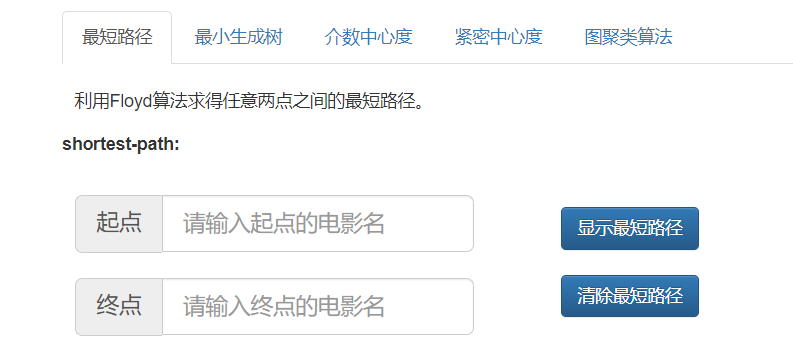
\includegraphics[width=0.6\linewidth]{../pictures/floyd}
	\caption{功能选择栏}
\end{figure}
\paragraph*{}
   下面我们将分别展示“最小生成树”,“最短路径”,“两种中心度计算”和提高算法:“社群发现”的可视化效果。从下页图中可以看到图聚类算法可以较为准确的划分社群,“团”的特征十分明显;其他基础功能的实现也比较准确和直观。在网页侧栏展示了论文和电影的基本信息,其中论文标题还提供了指向源网址的链接。更多细节请打开网页home.html查看。
\begin{center}
	\begin{figure}[ht] %强制单栏排版
		\centering %居中
		\begin{minipage}[b]{\linewidth} %整体划分一个0.93倍页面宽度的页面
			\begin{minipage}[b]{0.6\linewidth} %继续划分子页面 每个宽度0.17倍总宽度
				\centering
				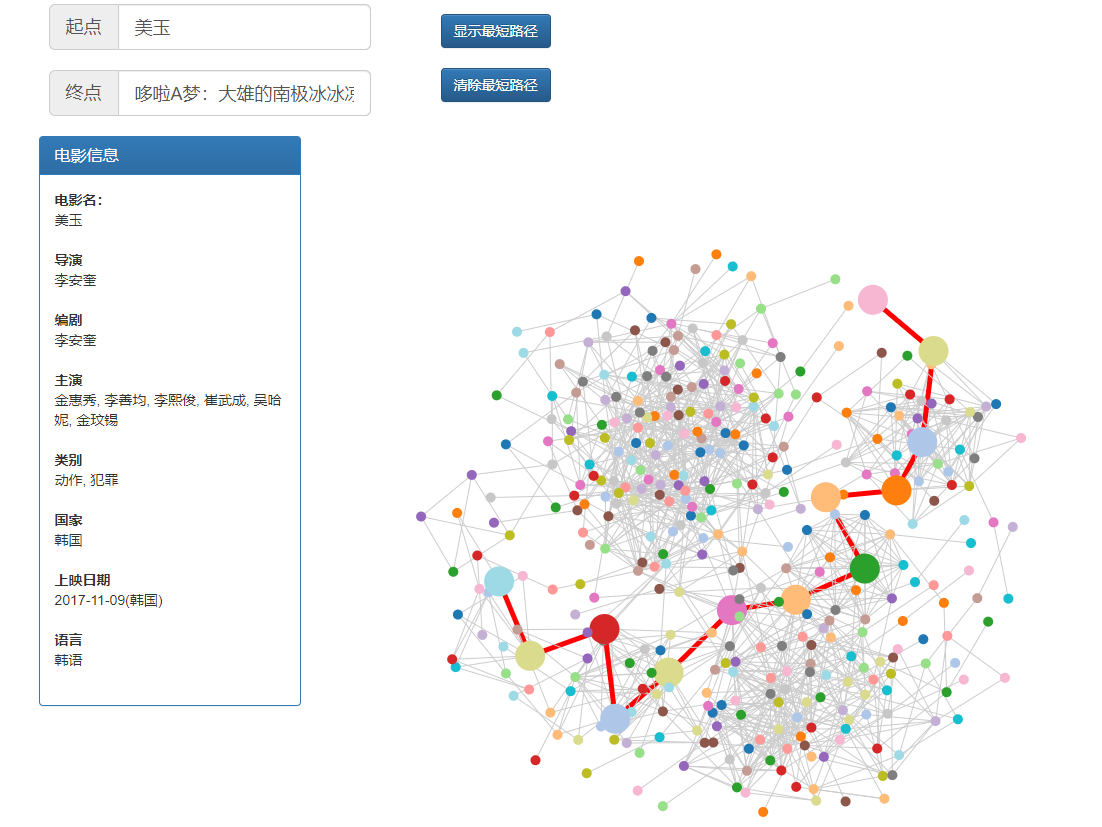
\includegraphics[width=\linewidth]{../pictures/show1}
				\caption{在输入框内输入起点和终点,可以高亮显示最短路径}
			\end{minipage}
			\hfill
			\begin{minipage}[b]{0.4\linewidth}
				\centering
				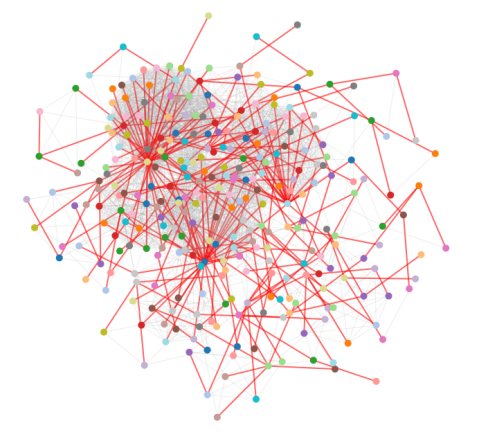
\includegraphics[width=\linewidth]{../pictures/show18}
				\caption{展示最小生成树}
			\end{minipage}
		\end{minipage}
	\end{figure}
\end{center}
\begin{center}
	\begin{figure}[ht] %强制单栏排版
		\centering %居中
		\begin{minipage}[b]{0.93\linewidth} %整体划分一个0.93倍页面宽度的页面
			\begin{minipage}[b]{0.46\linewidth} %继续划分子页面 每个宽度0.17倍总宽度
				\centering
				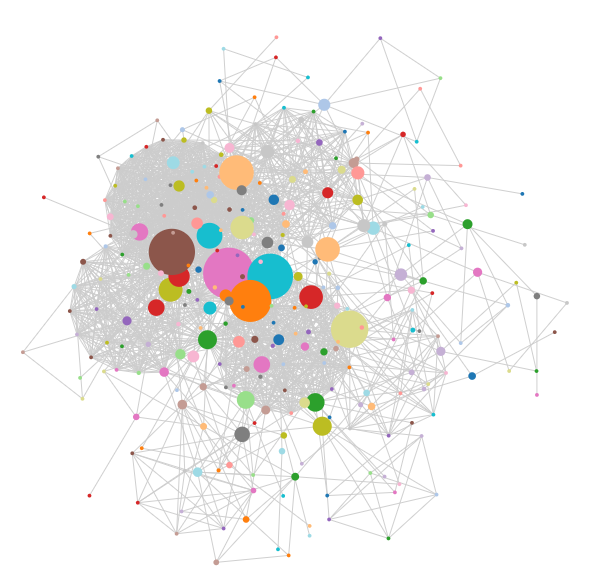
\includegraphics[width=\linewidth]{../pictures/show3}
				\caption{介数中心度展示}
			\end{minipage}
			\hfill
			\begin{minipage}[b]{0.46\linewidth}
				\centering
				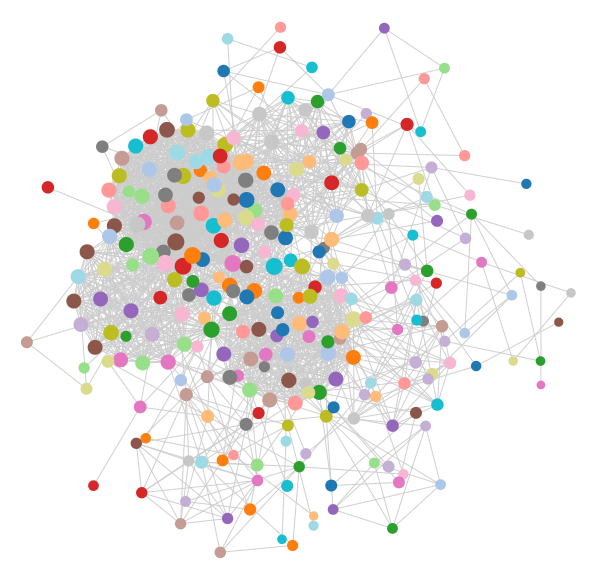
\includegraphics[width=\linewidth]{../pictures/show4}
				\caption{紧密中心度展示}
			\end{minipage}
		\end{minipage}
	\end{figure}
\end{center}
\begin{figure}[htb]
	\centering
	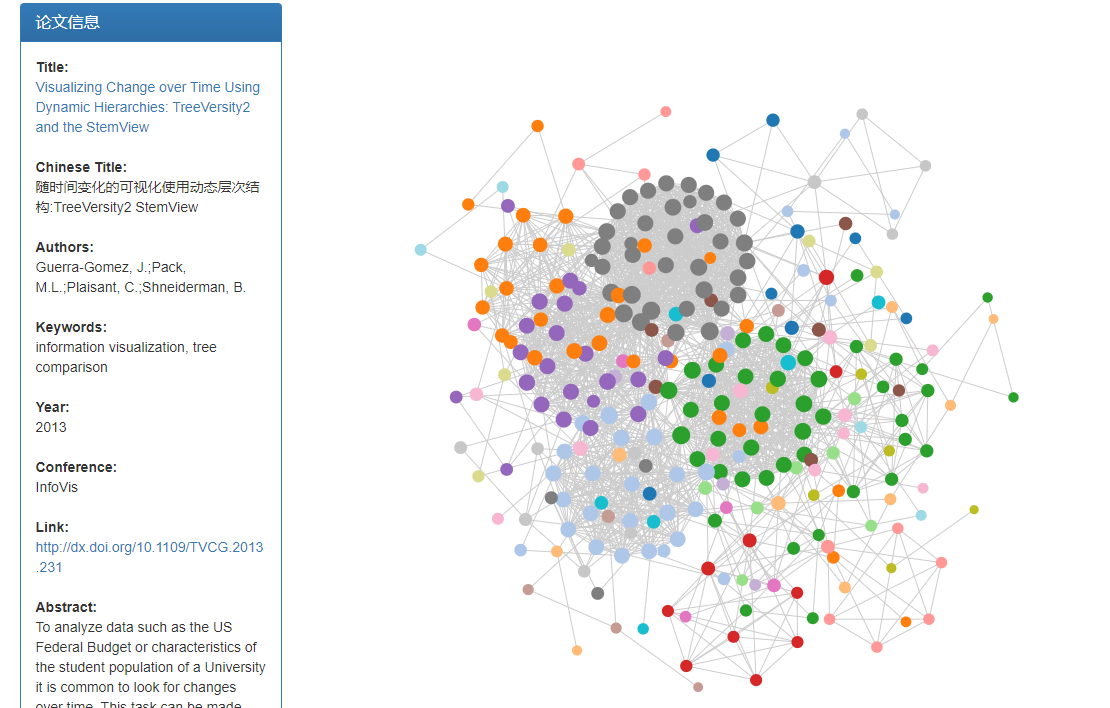
\includegraphics[width=0.8\linewidth]{../pictures/show5}
	\caption{展示图聚类算法}
\end{figure}
\clearpage

\ifx\allfiles\undefined
\end{document}
\fi

\section{算法概述}
下面介绍我们完成的算法,具体实现细节请参看cpp源文件中详细的注释。
\subsection{最小生成树}
最小生成树使用\textbf{基于堆优化的Prim算法},时间复杂度$O((n+e)logn)$. 我们也实现了基于并查集的Kruskal算法,仅保留在了cpp源文件中,在建模时并未使用。

最小生成树的总权值和树边等信息输出在程序运行日志中,因为该权值并不具有明确的物理意义,只代表节点之间联系的紧密程度。可视化的网页仅仅展示了最小支撑树的结构。
\subsection{任意两点最短路}
任意两点的最短路算法使用$O(n^3)$的\textbf{Floyd算法}。您在网页中输入起点和终点信息即可显示最短路。
\subsection{中心度算法}
\subsubsection{紧密中心度}
紧密中心度(Closeness Centrality)衡量了某一个节点和其它所有节点间最短路径距离之和;节点越中心,则距离之和越小,其倒数越大。简单地,对每个节点使用单源最短路算法\textbf{Dijkstra}即可计算某一个节点和其它所有节点间最短路径距离之和,复杂度$O(n^2\log n)$。最终我们使用\textbf{归一化的紧密中心度},即:
$$C_i = \frac{|V| - 1}{\sum_{j\neq i}d_{ij}}$$
\subsubsection{介数中心度}
介数中心度(Betweenness Centrality)用来衡量某一个节点出现在其他节点对间最短路径上的次数,节点位置越关键,则该指数越大。我们基于\textbf{Floyd算法}得出的结果统计“介数中心度”,先计算某一个节点出现在其他节点对间最短路径上的次数,复杂度$O(n^3)$。最终计算\textbf{归一化的介数中心度},即
$$B_i = \frac{count(i\quad occur\quad on\quad shortest\quad path)}{(n-1)(n-2) / 2}$$
\subsection{社群发现算法}
社群发现我使用\textbf{Fast-Unfolding算法}\cite{0803.0476},下面详细介绍一下。该算法以最优化图$G$的模块度(modularity)\cite{cond-mat/0308217}出发,定义如下:
\begin{equation}
\begin{aligned}
Q &= \frac{1}{2m}\underset{i,j\in 1,2,...n}{\sum}\left(A_{ij} - \frac{d_i d_j}{2m}\right)\delta(C_i, C_j)\\
&=\underset{i}{\sum}\left(\frac{d_{in}(C_i)}{2m} - \left(\frac{d_{tot}(C_i)}{2m}\right)^2\right)
\end{aligned}
\end{equation}
其中$d_{in}, d_{tot}$分别为某社区的总入度和总度数,$m$为边数,$A_{ij}$表示边权。

原文仅仅推导了从孤独节点加入社群的情况,我们对此进行了\textbf{推广},将问题一般化为“将节点$i$从社群$C_k$移出,移入社群$C_j$,对模块度$Q$的贡献”。简单推导后可以得到,将节点$i$从社群$C_k$移出,移入社群$C_j$,对模块度$Q$的贡献为:

\begin{equation}
\begin{aligned}
\triangle Q(i, C_j) &= \frac{1}{2m} \left[ \left(d_{in}(C_j) + d(k, C_j) - \frac{(d_{tot}(C_j)+d_k)^2}{2m}\right)+
\left( d_{in}(C_i) + d(k, C_i) - \frac{(d_{tot}(C_i)-d_k)^2}{2m} \right)\right]\\ 
&\qquad - \frac{1}{2m} \left[ \left( d_{in}(C_j) - \frac{d_{tot}(C_j)^2}{2m} \right) + 
\left( d_{in}(C_i) - \frac{ d_{tot} (C_i)^2 }{ 2m } \right) \right] \\
&= \frac{1}{2m}\left[d(C_j, k) - d(C_i, k) - \frac{2}{2m}\left(d_k \cdot(d_{tot}(C_j) - d_{tot}(C_i) + d_k)\right)\right]
\end{aligned}
\end{equation}
当节点$i$从社群$C_k$移出,移入社群$C_j$可以使得模块度增加时,我们进行此移动。此算法时间复杂度低,且对于大规模网络十分有效。但是此算法是输入敏感的,访问节点的顺序将影响最终的效果和收敛速度,所以我在/src/graph\_fastunfold.cpp中的实现采用了将节点shuffle之后重复运行若干次的做法,并使用OpenMP加速计算。

下面我们给出图的社群发现算法, Fast Unfolding\\
\begin{algorithm}[H]
	\caption{Fast Unfolding Algorithm}%算法名字
	%\LinesNumbered %要求显示行号
	\KwIn{$G=(V, E)$;}%输入参数
	\KwOut{clustering of $G$;}%输出
	$k = 0, G^0 = G$;\\ %\;用于换行
	\While{community partition (modularity) can still be changed (improved)}{
		make a simple clustering $C^k$ of $G^k$ such that $C_i^k = \{i\}$;\\
		\For{node $i \in G^k$}{
			remove the node $i$ from its community $C_i^k$;\\
			$C_N$ = set of neighbour communities of node $i$;\\
			$C_j^k = \arg\underset{C_{j'}^k\in C_N}{\max}\triangle Q(i, C_{j'}^k)$;\\
			\eIf{$\triangle Q(i, C_{j'}^k)>0$}
			{
				add node $i$ to the community $C_j^k$;
			}
			{
				leave node $i$ in the community $C_i^k$;
			}
		}
		build a new graph $G^{k+1}$ whose nodes are the communities of $C^k$;\\
		$k = k+1$;
	}
	make a clustering $C_{final}$ of $G$;\\
	\Return $C_{final}$
\end{algorithm}
从上面的展示可以看到,该算法的图聚类效果比较好。该算法的执行过程示意如下:
\begin{figure}[H]
	\centering
	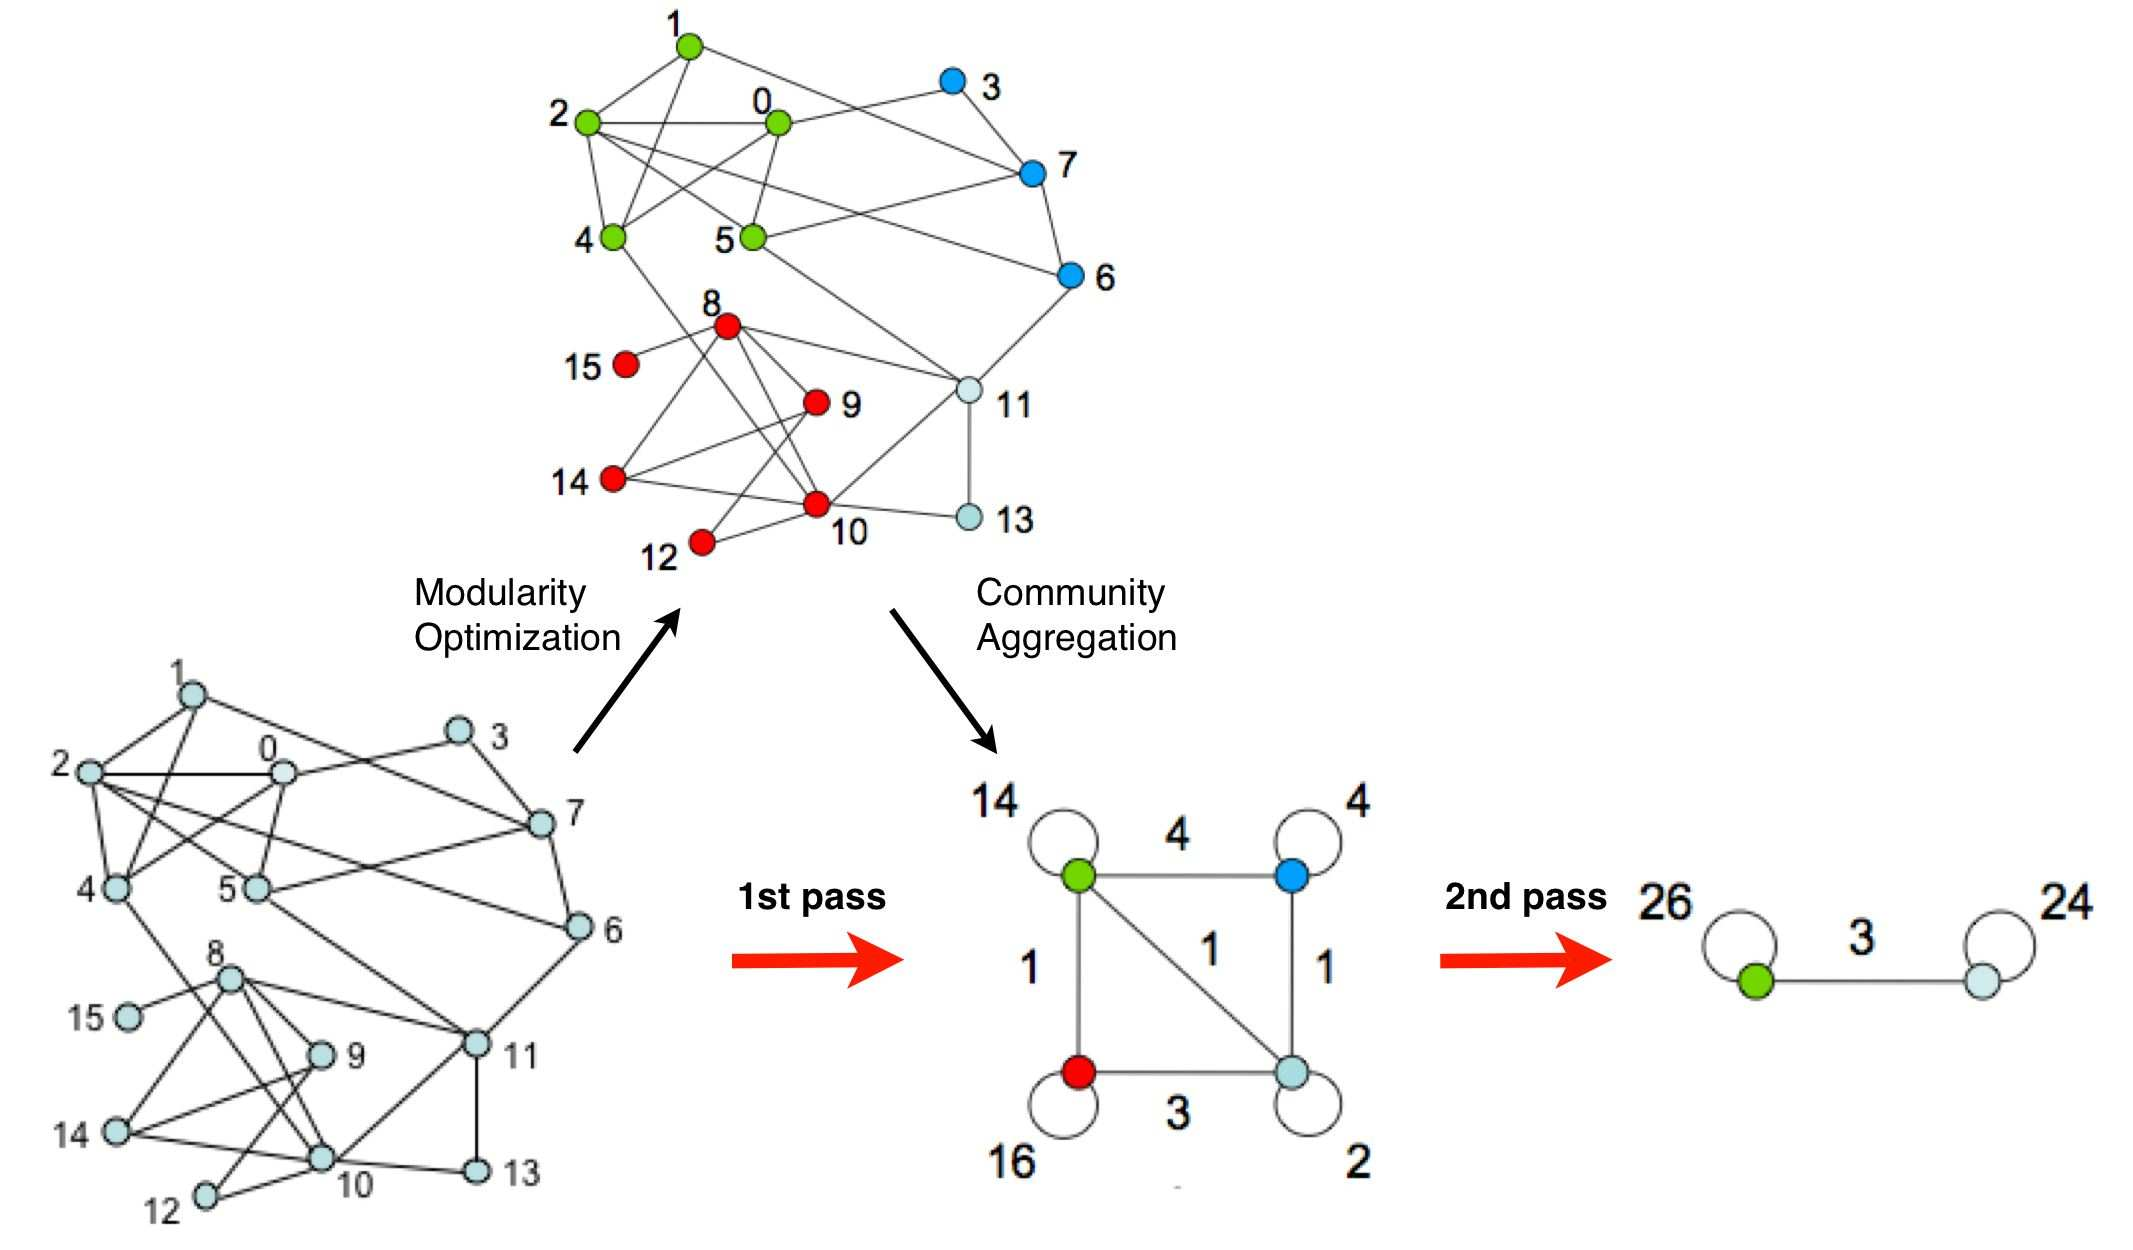
\includegraphics[width=0.7\linewidth]{../pictures/fastUnfolding}
	\caption{Fast-Unfolding算法}
\end{figure}
\section{电影数据集}
\subsection{建模方法}
    电影数据建模以电影为节点,以共同导演、编剧、演员建边,边权为$200/(10a+5b+c)$(a为是否是共同导演,是则为1,不是则为0;b为共同编剧数量,c为共同演员数量)。该权重可以看做两部电影或两个电影团队之间的相似度/关系度。
\subsection{相关统计数据}
    由于初始数据一共给出了4358部电影,规模过大,且图不连通,不方便分析,故选取了其中最大的连通分支,一共456部电影。从而,图的规模为456个节点、1228条边。
    
    图8展示了456个节点的度数分布情况,即不同度数的节点的个数。图9展示了电影建图的结果。
\begin{center}
    \begin{figure}[ht] %强制单栏排版
    \centering %居中
    \begin{minipage}[b]{0.95\linewidth} %整体划分一个0.93倍页面宽度的页面
    	\begin{minipage}[b]{0.47\linewidth} %继续划分子页面 每个宽度0.17倍总宽度
    	\centering
    	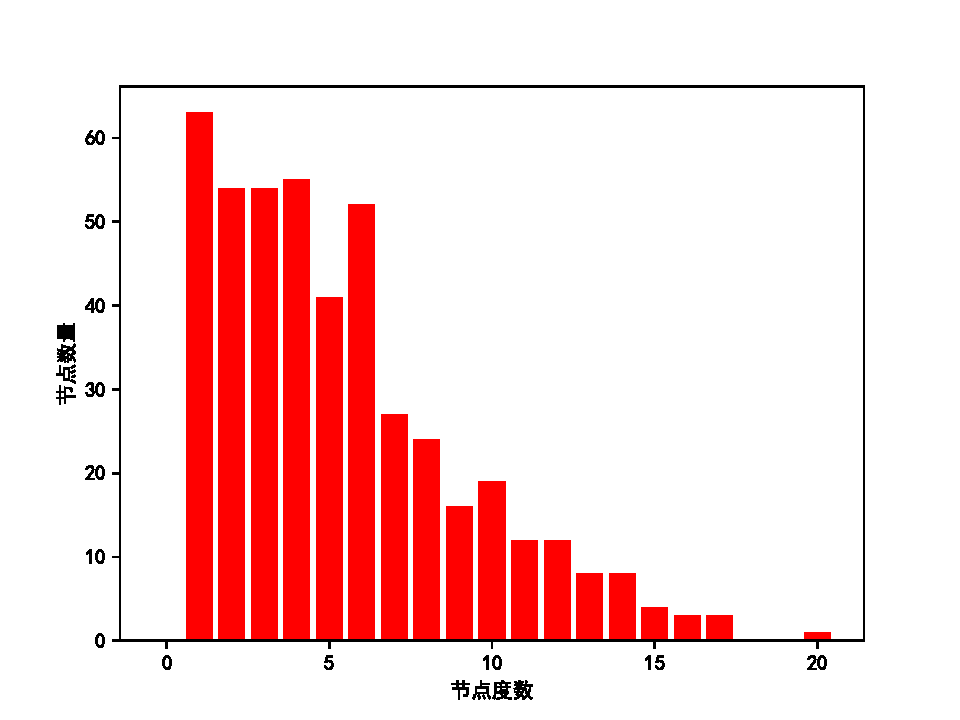
\includegraphics[width=\linewidth]{../pictures/movie_degree}
    	\caption{电影节点度数分布}
    	\end{minipage}
    	\hfill
    	\begin{minipage}[b]{0.46\linewidth}
    	\centering
    	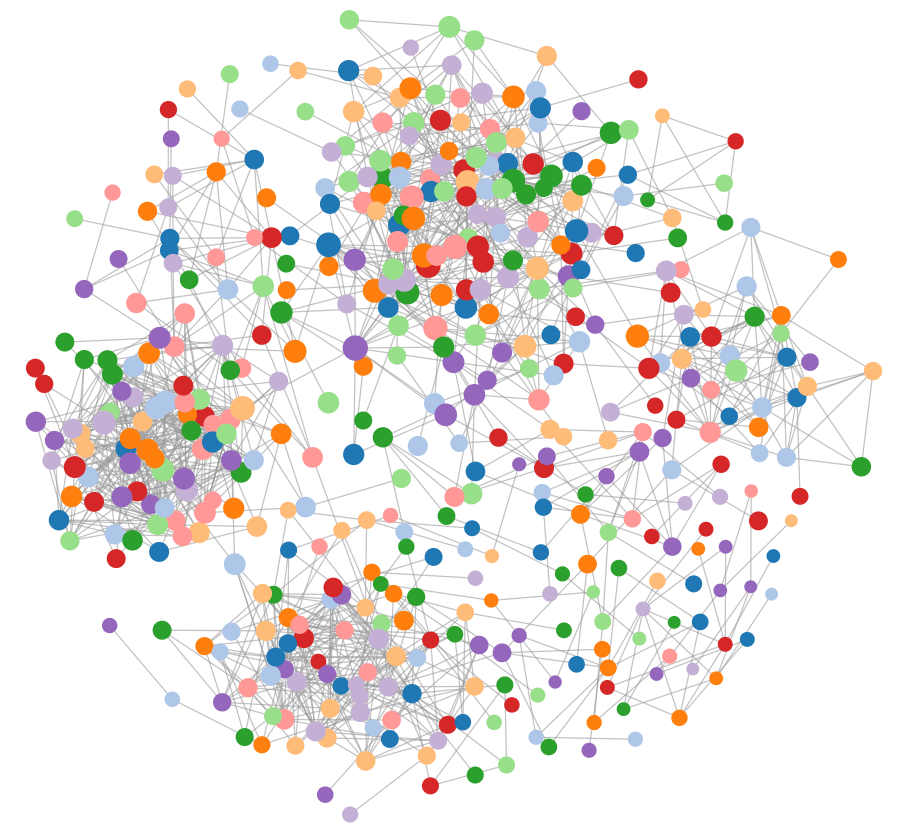
\includegraphics[width=\linewidth]{../pictures/show7}
    	\caption{电影建图结果}
    	\end{minipage}
    \end{minipage}
    \end{figure}
\end{center}
\subsection{算法实现与场景分析}
\subsubsection{最短路径}
    利用Floyd算法求得任意两点之间的最短路径。该最短路径的长度表明了两部电影之间的联系程度,路径越长则关联越小:如图10所示,该两个节点有相同编剧,距离较短;而如图11所示,该两个节点距离较长,关系度较小。
    
    \paragraph{场景分析}求最短路径可以用于电影网站的推荐算法:由于距离较短的节点有相同的导演或者相同的编剧,故在推荐电影的时候,可以在每一部电影下面推荐和这个电影代表的节点距离最小、且类别相同的10部电影。这样不仅保证了类别相同,也保证了导演、编剧的风格相近。
\begin{figure}[H]
	\centering
	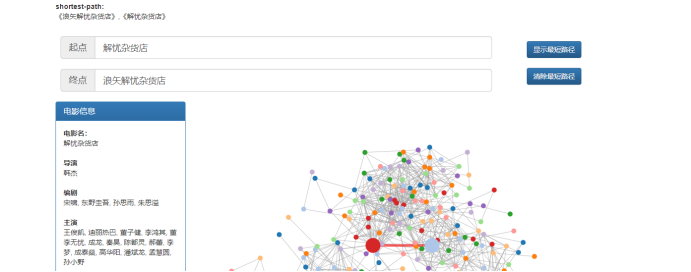
\includegraphics[width=0.6\linewidth]{../pictures/show8}
	\caption{《解忧杂货店》和《浪矢解忧杂货店》的最短路径}
\end{figure}
\begin{figure}[H]
	\centering
	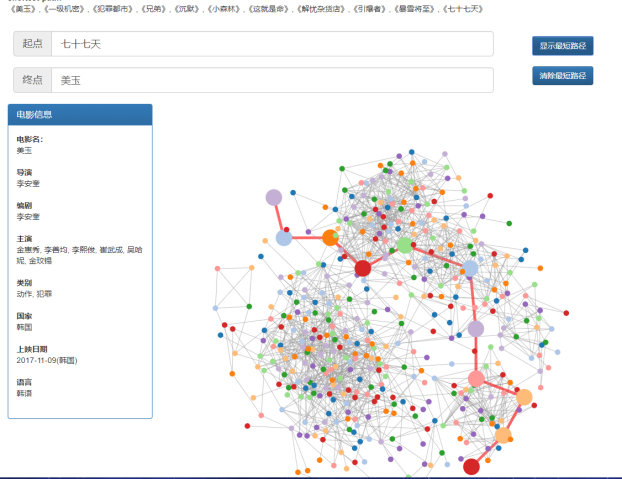
\includegraphics[width=0.6\linewidth]{../pictures/show9}
	\caption{《七十七天》和《美玉》之间的最短路径}
\end{figure}
\subsubsection{最小生成树}
	下图展示了最小生成树的结构。
	
    \paragraph{场景分析}我们对此构建了场景:如果要开一场电影节,需要者联系到所有拍摄这些电影的导演或者编剧,则可以利用该最小生成树,从某个节点开始,按照该最小生成树,依次去联系或说服导演。这样对于每一个导演来说,如果有经过合作的导演参加,则参与会议的积极性会提高,从而更好说服。
\begin{figure}[H]
	\centering
	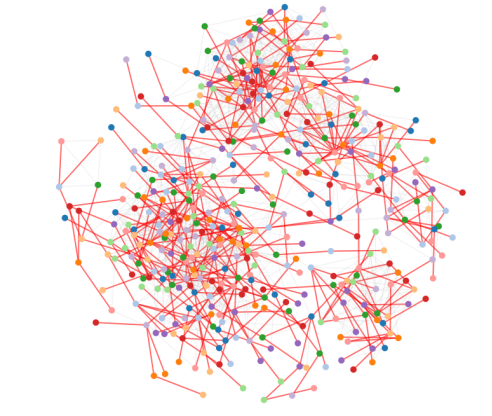
\includegraphics[width=0.6\linewidth]{../pictures/show10}
	\caption{电影所构建的图的最小生成树}
\end{figure}
\subsubsection{介数中心度}
    下图展示了介数中心度的可视化结果。 该图表明《解忧杂货店》等电影在该图当中的介数中心度较高。
    
    \paragraph{场景分析}介数中心度同样可以用于推荐。由于介数中心度高,故会更多的经过更多节点的最短路径,从而说明该节点可能是整个图的割点,或者该节点与其他节点的距离更短。从而对于这些电影,可以更方便的给出推荐算法,即通过这些推荐算法给出的电影和该部电影的相似度更高;同时如果是割点,也可能使得和该节点相邻的节点对应的电影能够跨越不同风格或者不同领域。在网站的首页,如果放一些介数中心度高的电影,虽然说可能并不是热门电影,对于电影网站的利益来讲,这样更有效的推荐算法和跨领域的电影更有利于增加该电影网站的点击量。如果电影要收费,用户愿意看更多的电影,也就能够获得更多的利润。
\begin{center}
	\begin{figure}[ht] %强制单栏排版
		\centering %居中
		\begin{minipage}[b]{0.95\linewidth} %整体划分一个0.93倍页面宽度的页面
			\begin{minipage}[b]{0.47\linewidth} %继续划分子页面 每个宽度0.17倍总宽度
				\centering
				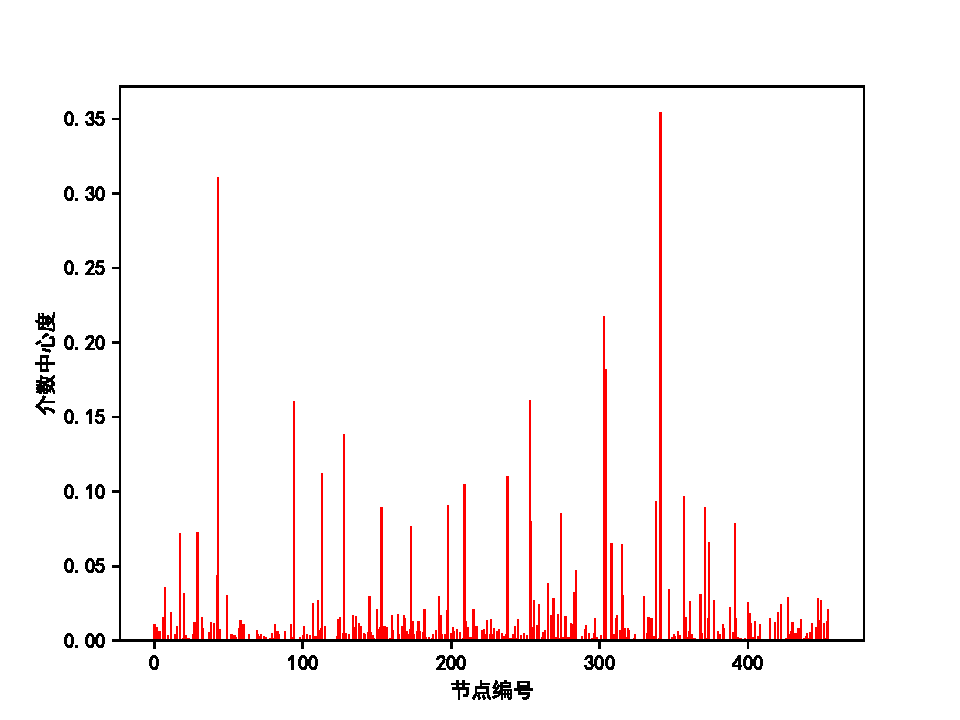
\includegraphics[width=\linewidth]{../pictures/movie_betweeness}
				\caption{电影节点介数中心度分布}
			\end{minipage}
			\hfill
			\begin{minipage}[b]{0.46\linewidth}
				\centering
				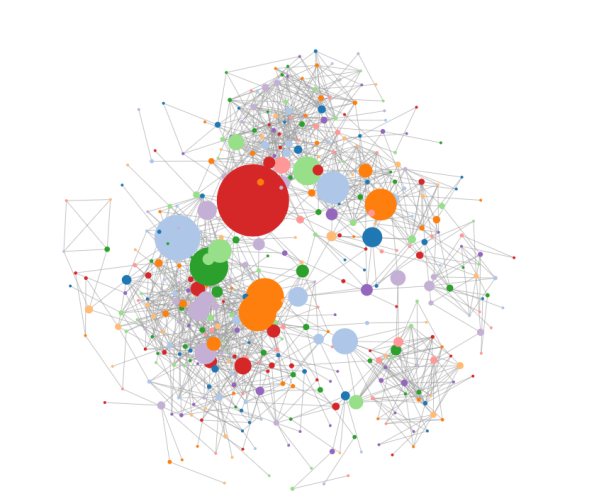
\includegraphics[width=\linewidth]{../pictures/show11}
				\caption{电影节点的介数中心度}
			\end{minipage}
		\end{minipage}
	\end{figure}
\end{center}
\subsubsection{紧密中心度}
    各个节点的紧密中心度分布如图15所示,建图结果如图16所示。
    
    \paragraph{场景分析}同6.3.2节,如果要开一场电影节,如果第一位联系的导演不受实际情况限制,则可以从紧密中心度最小的节点对应的导演开始,这样可以保证所花费的时间更小。因为在说服完成一位导演之后才可以继续去说服距离相近的电影所对应的导演。如果第一个导演对应节点的紧密中心度小,则可以在联系完成这位导演后迅速、并且并行的联系到其他的大量导演。同时,确保和其他节点的距离总和较小,也保证了最终的总用时较短。
\begin{center}
	\begin{figure}[ht] %强制单栏排版
		\centering %居中
		\begin{minipage}[b]{0.95\linewidth} %整体划分一个0.93倍页面宽度的页面
			\begin{minipage}[b]{0.47\linewidth} %继续划分子页面 每个宽度0.17倍总宽度
				\centering
				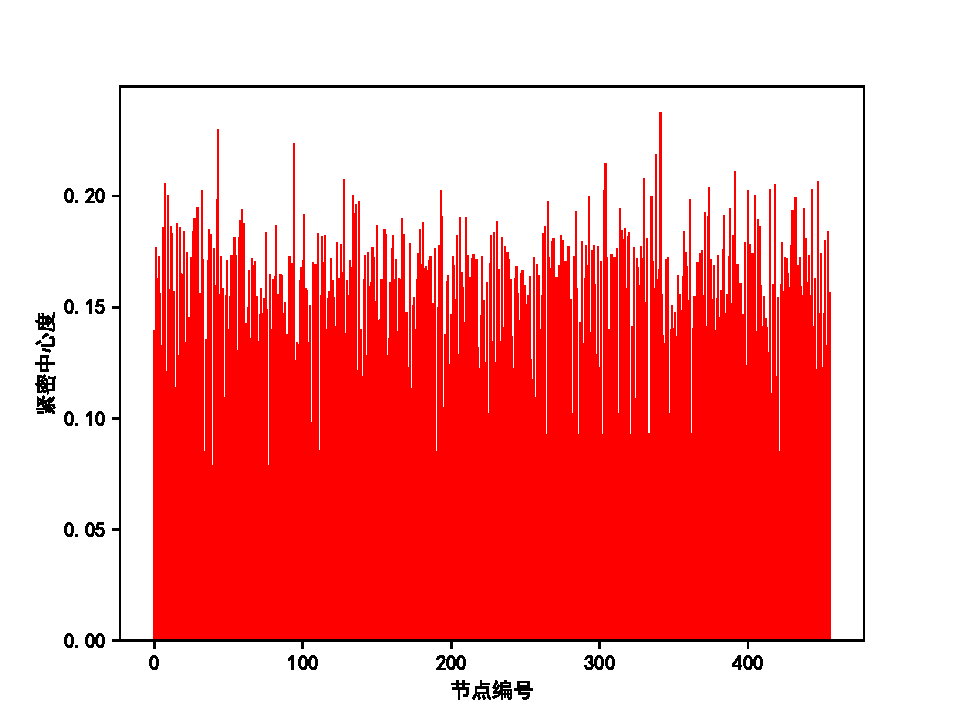
\includegraphics[width=\linewidth]{../pictures/movie_closeness}
				\caption{电影节点紧密中心度分布}
			\end{minipage}
			\hfill
			\begin{minipage}[b]{0.46\linewidth}
				\centering
				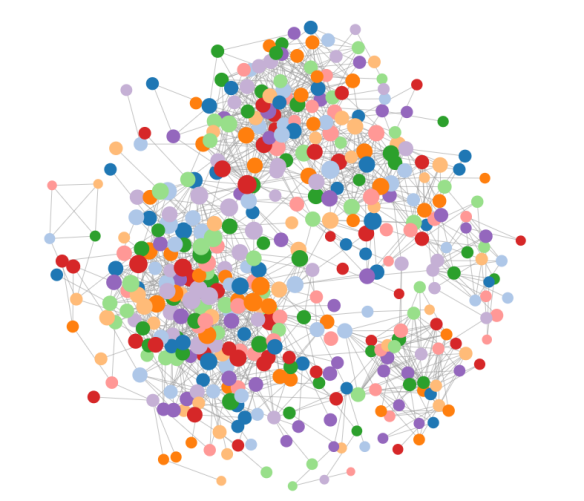
\includegraphics[width=\linewidth]{../pictures/show12}
				\caption{电影节点的紧密中心度}
			\end{minipage}
		\end{minipage}
	\end{figure}
\end{center}
\subsubsection{社区发现}
    使用Fast-Unfolding图聚类算法实现,详见第5节。图17显示的是整个图的图聚类算法的结果。这说明电影的导演之间合作交流较为密切, 我们明显的注意到,\textbf{电影社群与国家/地区密切相关}。进一步,如图18所示,处于同一个较大聚类的节点,其紧密中心度较小,且大致相同。
 
    \paragraph{场景分析} 如果要召开电影节,将导演不同风格、不同类型的众多导演召集到一块,这样在安排不同导演位置(例如酒店位置、就餐位置)的时候,可以将同一个聚类的导演安排到一块,这样就会让导演有更多话题可以交流;也可以有目的地将不同聚类的导演安排到一块,这样可以跨领域交流。
\begin{center}
	\begin{figure}[ht] %强制单栏排版
		\centering %居中
		\begin{minipage}[b]{0.95\linewidth} %整体划分一个0.93倍页面宽度的页面
			\begin{minipage}[b]{0.47\linewidth} %继续划分子页面 每个宽度0.17倍总宽度
				\centering
				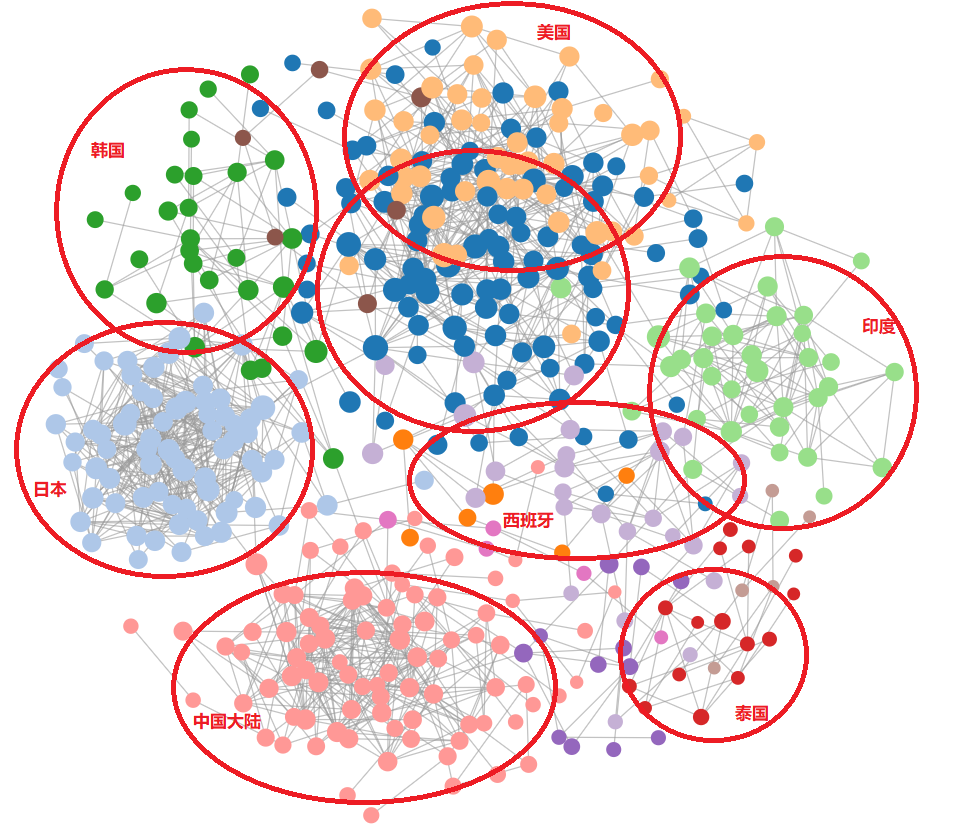
\includegraphics[width=\linewidth]{../pictures/new1}
				\caption{图聚类算法的结果,以及几个明显的聚类}
			\end{minipage}
			\hfill
			\begin{minipage}[b]{0.46\linewidth}
				\centering
				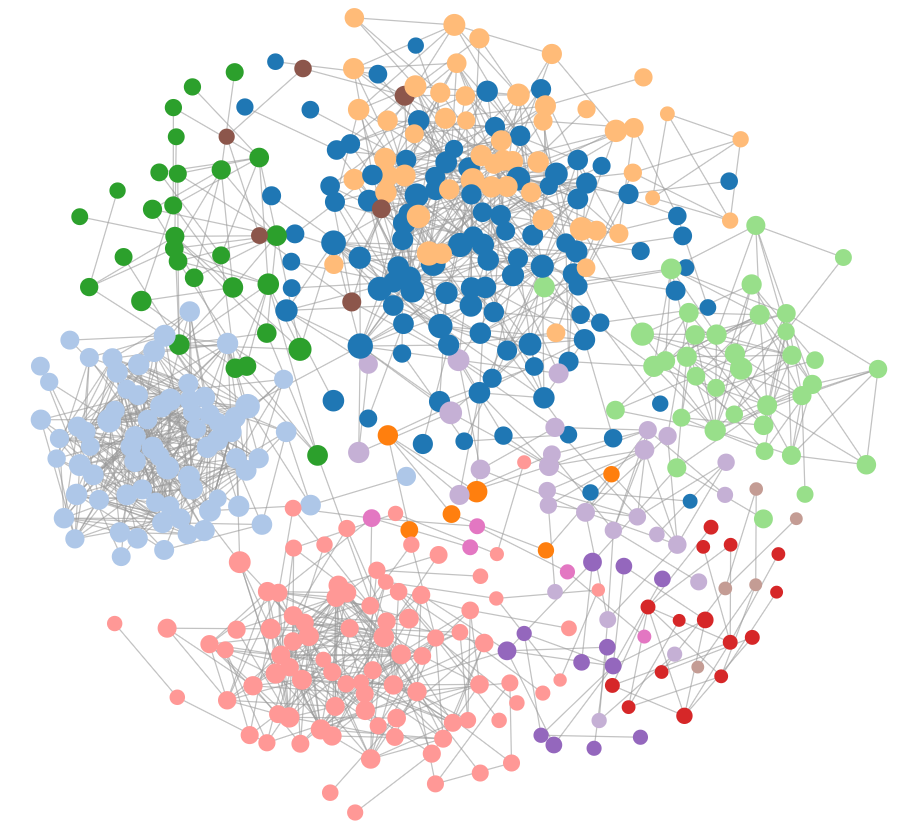
\includegraphics[width=\linewidth]{../pictures/new2}
				\caption{在图聚类算法的结果下看紧密中心度}
			\end{minipage}
		\end{minipage}
	\end{figure}
\end{center}
\section{论文数据集}
\subsection{建模方法}
    论文数据建模以论文为节点,以共同关键词(包括初始数据当中提供的第一作者等信息)建边,边权为$50/a$(a为相同关键词数)。该权重可以看做两个论文之间的相似度。同时提供了“有道翻译”的中文标题,便于理解。
\subsection{相关统计数据}
    由于初始数据一共给出了2752篇论文,规模过大,且图不连通,不方便分析,故选取了其中最大的连通分支,一共355篇。从而,图的规模为355个节点、2783条边。由此可见相比电影的图,论文的图更加密集。

    图19展示了节点的度数分布,图20展示了论文数据集的建图结果。
\begin{center}
	\begin{figure}[ht] %强制单栏排版
		\centering %居中
		\begin{minipage}[b]{0.95\linewidth} %整体划分一个0.93倍页面宽度的页面
			\begin{minipage}[b]{0.47\linewidth} %继续划分子页面 每个宽度0.17倍总宽度
				\centering
				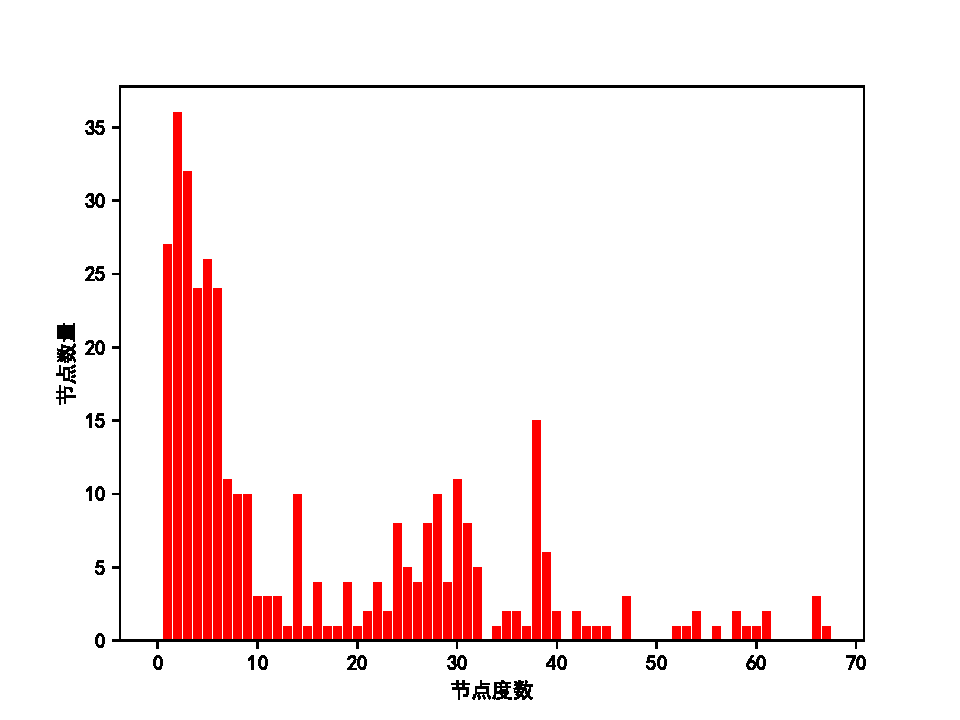
\includegraphics[width=\linewidth]{../pictures/paper_degree}
				\caption{论文节点度数分布}
			\end{minipage}
			\hfill
			\begin{minipage}[b]{0.46\linewidth}
				\centering
				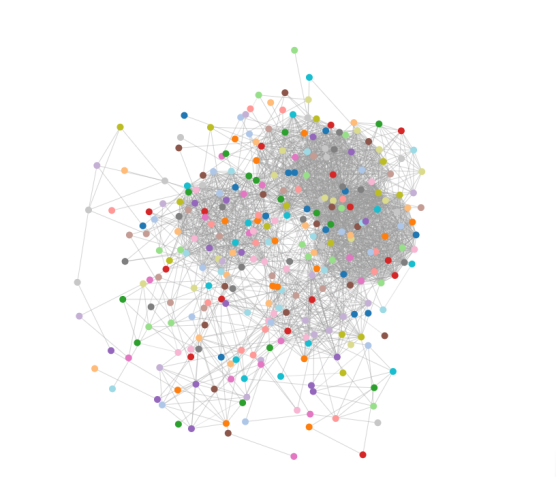
\includegraphics[width=\linewidth]{../pictures/show15}
				\caption{论文数据集的建图结果}
			\end{minipage}
		\end{minipage}
	\end{figure}
\end{center}
\subsection{算法实现与场景分析}
\subsubsection{最短路径}
    最短路径体现出了两篇论文,尤其是两篇没有相同关键词的论文的直接或间接的关联程度。两篇论文之间的最短路径越长,则说明论文之间的关系度越小。这可以用于相关论文的推荐。
    
    如图所示,图21所显示的两篇论文关系比较密切(有边直接连接),而图22所示的两篇论文关系则几乎没有什么联系。

    \paragraph{场景分析}求最短路径同样也可以运用于学术网站的推荐算法。对于一篇论文,读者读完了之后可能对该领域的研究情况还不甚了解。如果能够在该论文下面加一个相关链接,即推荐类似论文,读者将会更好了解该领域。
\begin{figure}[H]
	\centering
	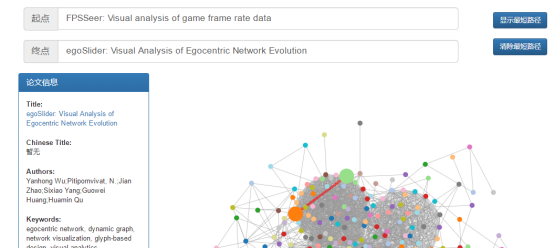
\includegraphics[width=0.6\linewidth]{../pictures/show16}
	\caption{两篇联系较为紧密的论文}
\end{figure}
\begin{figure}[H]
	\centering
	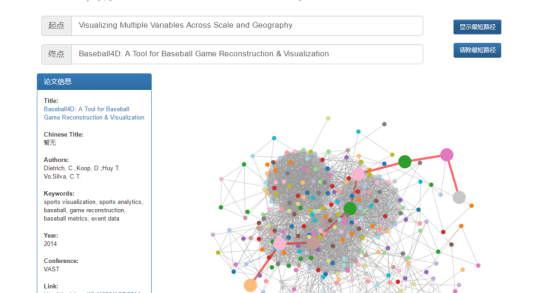
\includegraphics[width=0.6\linewidth]{../pictures/show17}
	\caption{两篇几乎没有联系的论文}
\end{figure}
\subsubsection{最小生成树}
    图的最小生成树如图23所示。
  
    \paragraph{场景分析}我们知道,计算机网络不能有环,如果有环,则会导致网络风暴。如果使用最小生成树,则避免了环的生成。这样在后续的其他论文处理当中,如果能够利用最小生成树,则可以大大降低图的边的数量,同时由于节点之间的距离较短,这样也保证里处理效率。
\begin{figure}[H]
	\centering
	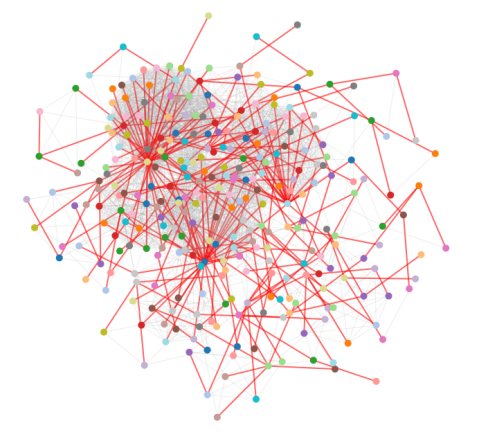
\includegraphics[width=0.6\linewidth]{../pictures/show18}
	\caption{论文节点组成图的最小生成树}
\end{figure}
\subsubsection{介数中心度}
    介数中心度分布如图24所示,建图结果如图25所示,介数中心度越大,该节点显示的大小越大。其中有大约10个节点的大小较为突出,在图中的中心度较高。
    
    \paragraph{场景分析}假如要办一场学术分享会,要邀请3-5位专家到场交流,介数中心度的值可以用于邀请专家。如果一篇论文在该图中的介数中心度较高,说明该论文在图中较重要,有可能是跨领域的,或者和更多的其他领域相关。如果能够邀请写这篇论文的作者,则该作者能够了解更多的领域(因为该论文和其他所有论文的相关性较高),从而能够在交流的时候获得更多的其它领域的拓展知识。
\begin{center}
	\begin{figure}[ht] %强制单栏排版
		\centering %居中
		\begin{minipage}[b]{0.95\linewidth} %整体划分一个0.93倍页面宽度的页面
			\begin{minipage}[b]{0.47\linewidth} %继续划分子页面 每个宽度0.17倍总宽度
				\centering
				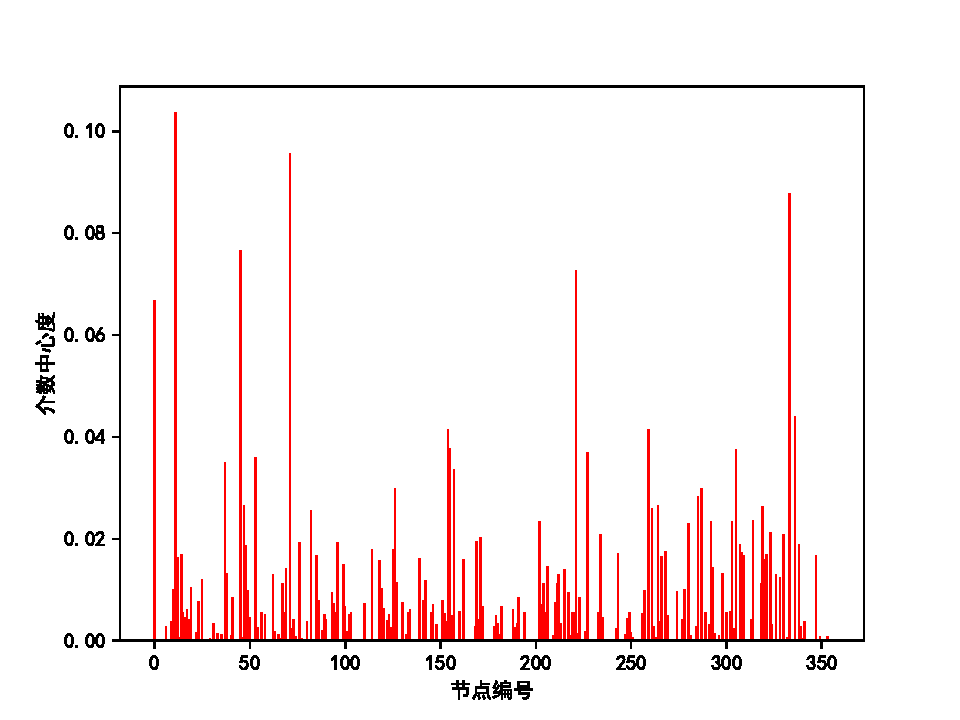
\includegraphics[width=\linewidth]{../pictures/paper_betweeness}
				\caption{论文节点介数中心度分布}
			\end{minipage}
			\hfill
			\begin{minipage}[b]{0.47\linewidth}
				\centering
				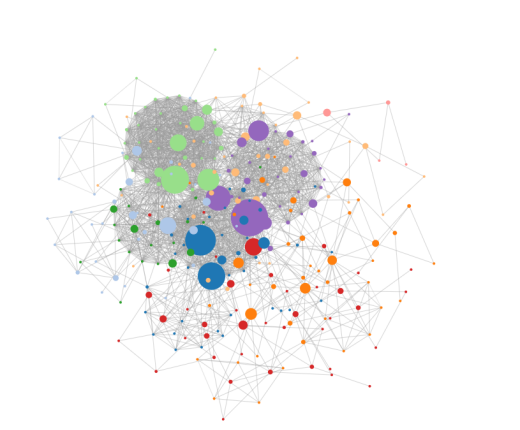
\includegraphics[width=\linewidth]{../pictures/show19}
				\caption{论文节点的介数中心度}
			\end{minipage}
		\end{minipage}
	\end{figure}
\end{center}
\subsubsection{紧密中心度}
    节点的紧密中心度分布如图26所示,建图结果如图27所示。紧密中心度越小,则该节点的大小越大。
    
    \paragraph{场景分析}同上面的介数中心度一样,紧密中心度的值也可以用于邀请专家(即邀请3-5位专家到场的情况)
\begin{center}
	\begin{figure}[ht] %强制单栏排版
		\centering %居中
		\begin{minipage}[b]{0.95\linewidth} %整体划分一个0.93倍页面宽度的页面
			\begin{minipage}[b]{0.47\linewidth} %继续划分子页面 每个宽度0.17倍总宽度
				\centering
				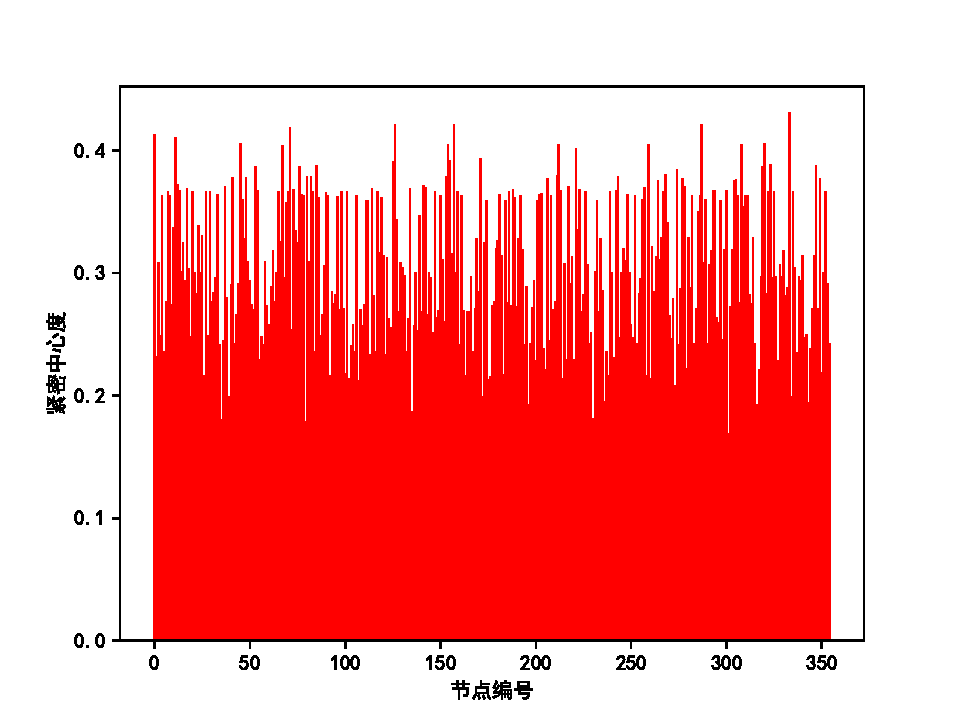
\includegraphics[width=\linewidth]{../pictures/paper_closeness}
				\caption{论文节点紧密中心度分布}
			\end{minipage}
			\hfill
			\begin{minipage}[b]{0.46\linewidth}
				\centering
				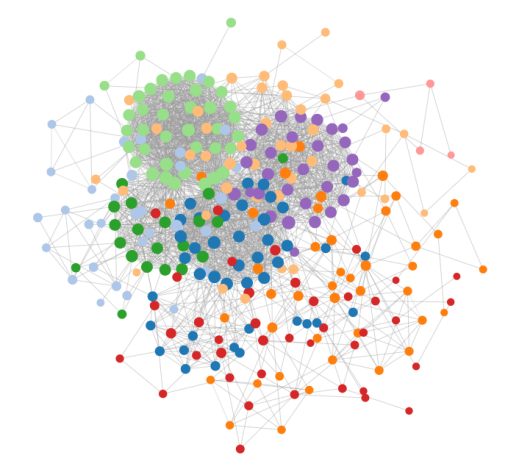
\includegraphics[width=\linewidth]{../pictures/show20}
				\caption{论文节点的紧密中心度}
			\end{minipage}
		\end{minipage}
	\end{figure}
\end{center}
\subsubsection{社区发现}
    图28显示的是整个图的图聚类算法的结果。由于该图相比电影的图更加密集,故一些小的聚类不能从图中明显看出,但仍然有6个点数较多的聚类。这说明这些论文处于同一个领域,且作者之间合作交流较为密切。进一步,如图29所示,处于同一个较大聚类的节点,其紧密中心度较小,且大致相同。
    
    \paragraph{场景分析}假如要办一场学术研讨会,并且大量学者要到场,则图聚类算法可以用于安排到场学者的住处和就坐位置。可以安排同一个领域的学者在一块,这样能够促进同一个领域的学术交流;也可以可以安排不同领域的学者在一块,这样可以促进跨领域沟通。
\begin{center}
	\begin{figure}[ht] %强制单栏排版
		\centering %居中
		\begin{minipage}[b]{0.95\linewidth} %整体划分一个0.93倍页面宽度的页面
			\begin{minipage}[b]{0.47\linewidth} %继续划分子页面 每个宽度0.17倍总宽度
				\centering
				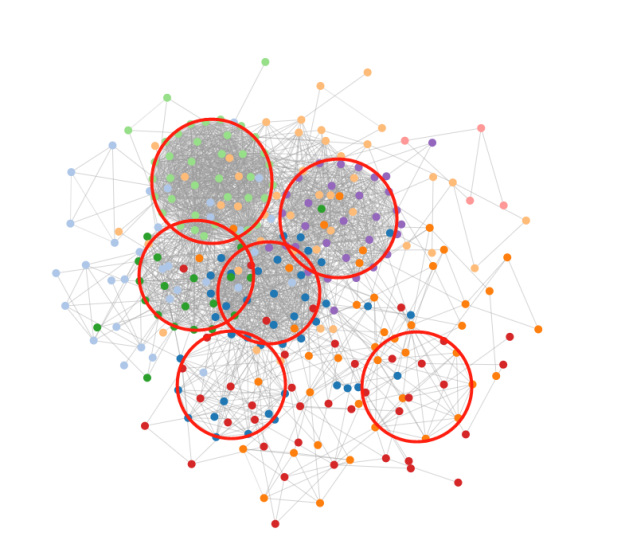
\includegraphics[width=\linewidth]{../pictures/show21}
				\caption{图聚类算法结果和几个明显的聚类}
			\end{minipage}
			\hfill
			\begin{minipage}[b]{0.46\linewidth}
				\centering
				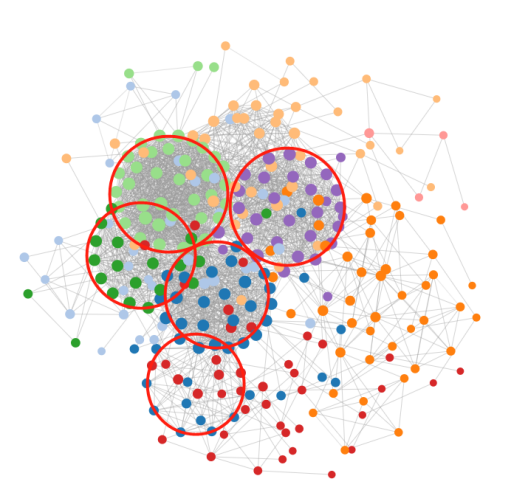
\includegraphics[width=\linewidth]{../pictures/show22}
				\caption{在图聚类算法下看紧密中心度}
			\end{minipage}
		\end{minipage}
	\end{figure}
\end{center}
\section{总结}
    本次大作业完成了对电影数据集、论文数据集的整理,并取出了两个数据集的最大连通分支,从最短路径、最小生成树、介数中心度、紧密中心度、社区发现等5个角度进行数据分析,较为直观地展示了不同电影/论文之间的联系程度,以及电影/论文节点在图中的重要程度。在学了大半个学期的图论理论知识之后,这次大作业是对这些理论知识的一个很好的应用,如Floyd算法、dijkstra算法以及难度较大的社群发现算法等;同时,也接触了介数中心度、图聚类等新概念,对已学知识进行了一些扩展。通过这些应用,也体会到了图论在计算机科学当中的应用价值。
    
    此外,这次大作业也让我们新接触了数据可视化、web编程等今后要频繁使用的工具。通过对这些的熟悉,也为今后的学习、使用和开发打下了基础。
    
    疫情期间的学习给我们带来了新的挑战,但也留下了难忘的回忆。老师和助教们的帮助和支持化解了居家学习的不便,在此向老师和助教的辛勤付出表示感谢!

\bibliographystyle{ieeetr}
\bibliography{ref.bib}

\appendix
\section{Python Networkx图聚类结果}
\begin{center}
	\begin{figure}[ht] %强制单栏排版
		\centering %居中
		\begin{minipage}[b]{0.95\linewidth} %整体划分一个0.93倍页面宽度的页面
			\begin{minipage}[b]{0.47\linewidth} %继续划分子页面 每个宽度0.17倍总宽度
				\centering
				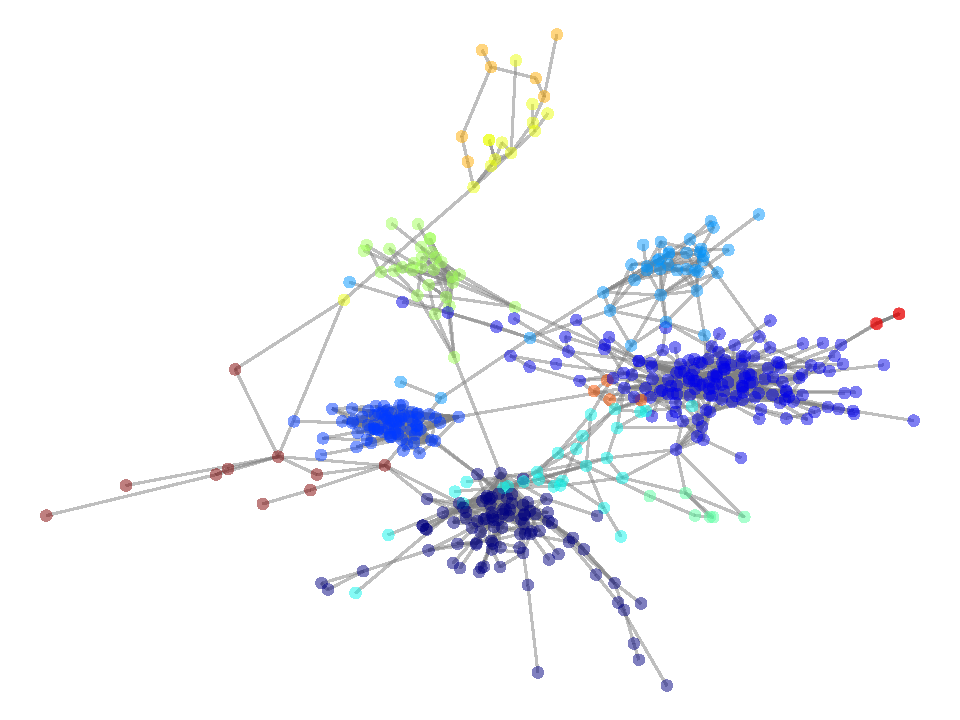
\includegraphics[width=\linewidth]{../pictures/movie_graph}
				\caption{电影数据集}
			\end{minipage}
			\hfill
			\begin{minipage}[b]{0.46\linewidth}
				\centering
				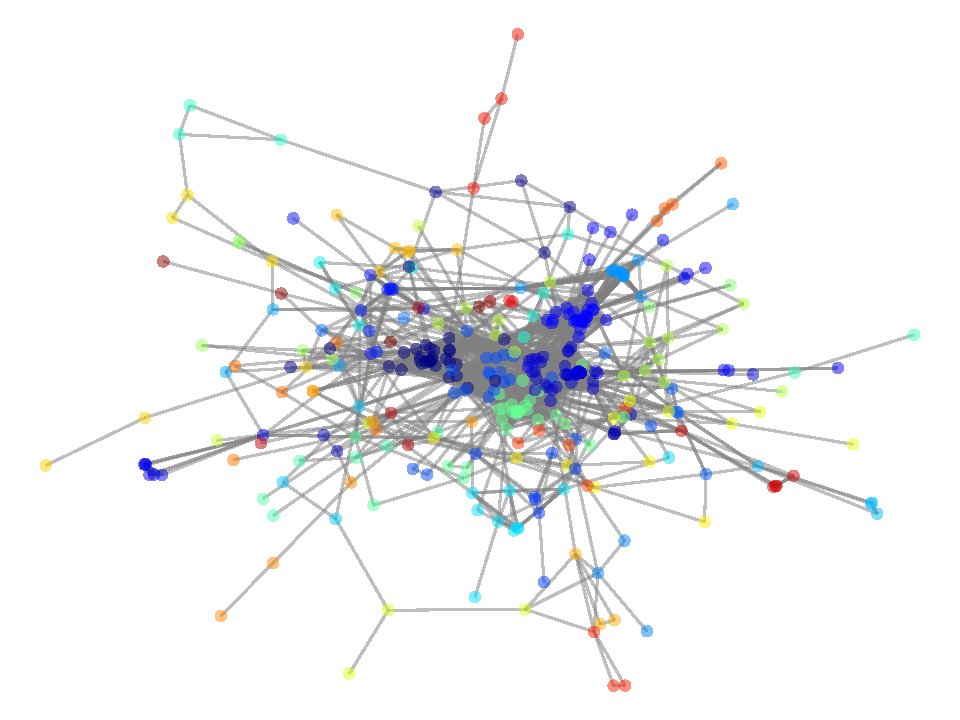
\includegraphics[width=\linewidth]{../pictures/paper_graph}
				\caption{论文数据集}
			\end{minipage}
		\end{minipage}
	\end{figure}
\end{center}
\end{document}